% ODD: MODULE 1
% EVEN: MODULE 3

\ifnum \Version=1

\part A plane curve $\mathbf r(t)$ has curvature $\kappa = \frac{1}{4}$ at $\mathbf r(t_0) = \langle 5, 3 \rangle$, and the unit normal vector at $t=t_0$ is $\mathbf  N = \mathbf j = \langle 0, 1 \rangle$. The equation of the osculating circle at $t=t_0$ is \framebox{\strut\hspace{3.5cm}}.

\ifnum \Solutions=1 {\color{DarkBlue} \textit{Answer:} \textit{Solutions:} Recall that The circle of curvature, or osculating circle, at a point $P$ on a plane curve where $\kappa \ne 0$ is the circle in the plane of the curve that

\begin{enumerate}
    \item is tangent to the curve at P (has the same tangent line the curve has)
    \item has the same curvature the curve has at P
    \item lies toward the concave or inner side of the curve
\end{enumerate}
The \textbf{radius of curvature} of the curve at P is the radius of the circle of curvature, which is $\frac{1}{\kappa}$. So to obtain the radius, we calculate $\kappa$ and take the reciprocal. The \textbf{center} of the osculating circle of the curve at P lies on the inner side of the curve, and the unit normal points in the direction of the inner side of the planar curve. 

So for this problem we have a circle with radius $1/\kappa = 4$, and whose centre is 4 units away from the point $(5,3)$ in the direction of $\mathbf N$. The circle has equation
$$(x-5)^2 + (y-7)^2 = 4^2$$
} 
\else
  
\fi        
\fi



% AVERAGE VALUE AND TRIANGULAR REGION
\ifnum \Version=2
    \part The average value of $f(x,y) = 12-8xy$ over the region in the first quadrant bounded by $x=0$, $y=0$, and $y=4-2x$ is $\displaystyle  \int_a^b \int_c^d g(x,y) \, dx \, dy$,  where $a=\framebox{\strut\hspace{1cm}}$, $b=\framebox{\strut\hspace{1cm}}$, $c=\framebox{\strut\hspace{2cm}}$, $d=\framebox{\strut\hspace{2cm}}$, and $g(x,y) = \framebox{\strut\hspace{2cm}}$.

    \ifnum \Solutions=1 
    {\color{DarkBlue} 
    The average value of a function $f(x,y)$ over a region $R$ is given by 
    \begin{align}
        \text{Average value of }f\text{ over region }R &= \frac{1}{\text{area of region }R}\iint_R f \, dA \\&= \iint_R \frac{f(x,y)}{\text{area of region }R} \, dA
    \end{align}
    Therefore to obtain $g(x,y)$ we can calculate
    \begin{align}
        g(x,y) = \frac{f(x,y)}{\text{area of region }R}
    \end{align}
    So we need the area of the region. It can help to sketch the region, as shown in the diagram below. 
       \begin{center}     
        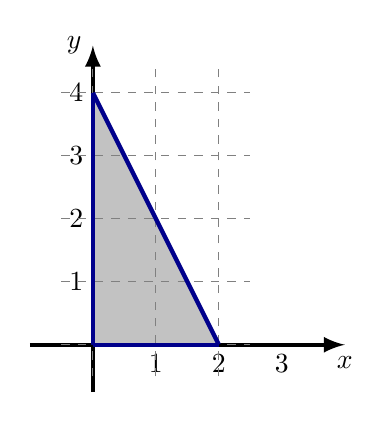
\begin{tikzpicture}[scale=0.8]
        \draw[fill=gray!80!black, opacity=0.4] (0,0) -- (0,4) -- (2,0);        
        \draw[ultra thick,->,>=latex] (-1,0)--(4,0) node[below] {$x$};
        \draw[ultra thick,->,>=latex] (0,-0.75)--(0,4.75) node[left] {$y$};
        \draw (1,0) node[below] {$1$};          
        \draw (2,0) node[below] {$2$};          
        \draw (3,0) node[below] {$3$};          
        \draw (0,1) node[left] {$1$};        
        \draw (0,2) node[left] {$2$};
        \draw (0,3) node[left] {$3$};
        \draw (0,4) node[left] {$4$};
        \draw[help lines,gray,thin,dashed] (-0.5, -0.5) grid (2.5, 4.5);
        \draw[domain=0:2,ultra thick,DarkBlue,samples=200] plot ({\x},{4-2*\x });
        \draw[domain=0:2,ultra thick,DarkBlue,samples=200] plot ({\x},{0 });
        \draw[ultra thick,-,DarkBlue,>=latex] (0,0)--(0,4);
    \end{tikzpicture}
    \end{center}     
    The region is bounded on the \textbf{right} by $y=4-2x$, or $x=2-y/2$. The region is also bounded on the \textbf{left} by $x=0$. The region is 
    $$R = \{(x,y) \in \mathbb R^2 \, | \, 0\le y \le 4, \ 0 < x < 2-y/2\}$$
    The area of the region is half the area of the rectangle whose length is 2 and height is 4. 
    $$\text{area of triangular region} = \frac12 ( 2 \cdot 4) = 4$$    
    Therefore, 
    \begin{align}
        a & = 0 \\
        b &= 4 \\
        c &= 0 \\
        d &= 2-y/2 \\
        g &= \frac{12-8xy}{4} = 3 - 2xy
    \end{align}
    }
   \else

   \fi
\fi 




\ifnum \Version=3

\part The plane that passes through $P(1,3,2)$ and contains the line $x=1+t$, $y=2+3t$, $z=2+2t$ is \framebox{\strut\hspace{4cm}}. The distance between the point $P$ and the $x$-axis is \framebox{\strut\hspace{1cm}}. 

\ifnum \Solutions=1 {\color{DarkBlue} \textit{Solutions:} The plane is parallel to direction vector of given line, $\mathbf  v = \langle 1,3,2\rangle$. Line contains $Q(1,2,2)$, so the plane is also parallel to the vector $\mathbf{PQ} = \langle 1,2,2 \rangle - \langle 1,3,2 \rangle = \langle 0,-1,0 \rangle$. It would also be ok to use any scalar multiple of this. \\[12pt]
A normal to the plane is $$\mathbf n = \mathbf  v \times \mathbf {PQ} = \begin{vmatrix} i & j & k \\ 1&3&2 \\ 0&-1&0\end{vmatrix} = \langle 2,0,-1\rangle = 2\mathbf i-\mathbf k$$ So using point $P(1,3,2)$ and $\mathbf n$, the plane has equation \begin{align}
    (2)(x-1)+(0)(y-3) + (-1)(z-2) = 0 
\end{align}which could be simplified to other forms, such as $$2x-z=0$$ But it isn't necessary to simplify the equation. The distance between the point and the $x$-axis is $\sqrt{3^2+2^2} = \sqrt{13}$.
}
\else
  
\fi
\fi



\ifnum \Version=4
% SHORT SPHERICAL AND CYLINDRICAL EXERCISE
% VERBATUM FROM SPRING 2022 QUIZ
% hand written solution only
\part Point $P$ has rectangular (Cartesian) coordinates $(x,y,z) = (0,-3,4)$ in $\mathbb R^3$. In cylindrical coordinates, the point is $(r,\theta,z)$, and in spherical coordinates the point is $(\rho, \phi, \theta)$. Where $r=\framebox{\strut\hspace{1cm}}$, $\theta=\framebox{\strut\hspace{1cm}}$, $z=\framebox{\strut\hspace{1cm}}$, $\rho=\framebox{\strut\hspace{1.5cm}}$, and $\phi=\framebox{\strut\hspace{3cm}}$. 

    \ifnum \Solutions=1 {\color{DarkBlue} \textit{Solutions:} To convert to cylindrical we can use the equation $r^2 = x^2 + y^2$. 
    \begin{align}
        r^2 &= x^2 + y^2 = 0^2 + (-3)^2 = 9 \ \Rightarrow \ r = 3 
    \end{align}
    To determine $\theta$ we notice that $P$ lies on the $y-$axis and has a negative $y$ value. So $\theta = 3\pi/2$.
    $$\displaystyle (r,\theta,z) = (3,\frac{3\pi}2,4)$$
    In spherical, we can start by obtaining $\rho$. 
    \begin{align}
        \rho^2 &= x^2+y^2+z^2\\
        \rho^2 &= 0^2 + (-3)^2 + 4^2 = 25 \\
        \rho &= 5 
    \end{align}
    To obtain $\phi$ we can use the equation that relates $y$ to spherical. Using the expression for $y$, and the values that we already have for $y$, $\rho$ and $\theta$:
    \begin{align}
        y &= \rho \sin\phi \sin\theta \\
        -3 &= 5\sin\phi \sin(3\pi/2) \\
        3 &= 5\sin\phi \\
        \sin\phi &= 3/5 \\
        \phi &= \arcsin (3/5)
    \end{align}
    Our coordinates in spherical are
    \begin{align}
        \rho &= 5\\
        \phi &= \arcsin (3/5)\\
        \theta &= \frac{3\pi}2  
    \end{align}
    Note the following.
    \begin{itemize}
        \item Note that we could also obtain $\phi$ using a right-angle triangle in the $yz-$plane. 
        \item Other similar approaches can lead to other equivalent expressions for $\phi$, such as $\phi = \arctan(3/4)$.
        \item Our particular textbook uses the convention $(\rho, \phi, \theta)$, not $(\rho, \theta,\phi)$.
    \end{itemize}
    } 
    \else
      
    \fi
    
\fi

\ifnum \Version=5
\part The velocity vector of an object moving on the curve $\mathbf r(t)$ is $\mathbf v(t) = \langle 3\cos (2t), 3\sin (2t) \rangle$ for $t>0$. The speed of the object for $t>0$ is $s(t) = |\mathbf v | = \framebox{\strut\hspace{1.5cm}}$. The unit tangent vector for $t>0$ is $\mathbf T = \langle f(t), g(t)  \rangle$, where $f(t) = \framebox{\strut\hspace{2cm}}$, and $g(t) = \framebox{\strut\hspace{2cm}}$.  The curvature for $t>0$ is \framebox{\strut\hspace{1.5cm}}. 

\ifnum \Solutions=1 {\color{DarkBlue} \textit{Answer:} \textit{Solutions:} The speed is the magnitude of the given velocity vector and is
\begin{align}
    s &= |\mathbf v | =  \sqrt{(3\cos t)^2 + (3\sin t)^2  } = \sqrt{3^2 (\cos ^2 t + \sin^2 t) + 3^2} = \sqrt{ 9} = 3
\end{align}
The unit tangent vector is 
\begin{align}
    \mathbf T &= \frac{\mathbf v}{|\mathbf v|} 
    = \langle \frac{3}{3}\cos(2 t) , \frac 33 \sin (2t) \rangle 
    = \langle \cos(2 t) ,  \sin (2t) \rangle
\end{align}
For curvature we also need
\begin{align}
    \frac{d\mathbf T}{dt } &= \langle -2 \sin 2t, 2 \cos 2t\rangle \\
    \left | \frac{d\mathbf T}{dt } \right| &= \sqrt{ \left(-2\sin 2t\right)^2 +   \left(2 \cos 2 t\right)^2 } = 2
\end{align}
The curvature is
\begin{align}
    \kappa = \frac{1}{|\mathbf v |}\left| \frac{d\mathbf T}{dt}\right| = \frac{1}{3} \cdot 2 = \frac{2}{3}
\end{align}
} 
\else
\fi        
\fi




% SIDEWAYS PARABOLA AND A LINEAR
\ifnum \Version=6
    \part The area of the region bounded by $x=-y^2$ and $y=x+2$ is $\displaystyle  \int_a^b \int_c^d f(x,y) \, dx \, dy$,  where $a=\framebox{\strut\hspace{1cm}}$, $b=\framebox{\strut\hspace{1cm}}$, $c=\framebox{\strut\hspace{2cm}}$, $d=\framebox{\strut\hspace{2cm}}$, and $f(x,y) = \framebox{\strut\hspace{2cm}}$.
    
    \ifnum \Solutions=1 
    {\color{DarkBlue} We want to determine where the two curves intersect. Setting them equal to each other: 
    \begin{align}
        -y^2 &= y - 2 \\
        0 &= y^2 + y - 2 \\
        0 &= (y+2)(y-1) \\
        y &= -2, 1
    \end{align}
    To obtain the $x-$coordinates, we can use either curve. Substituting the two $y-$values into either curve gives us two intersection points
    $$(-4,-2), (-1,1)$$
    It can help to sketch the two curves, as shown in the diagram below. 
       \begin{center}     
    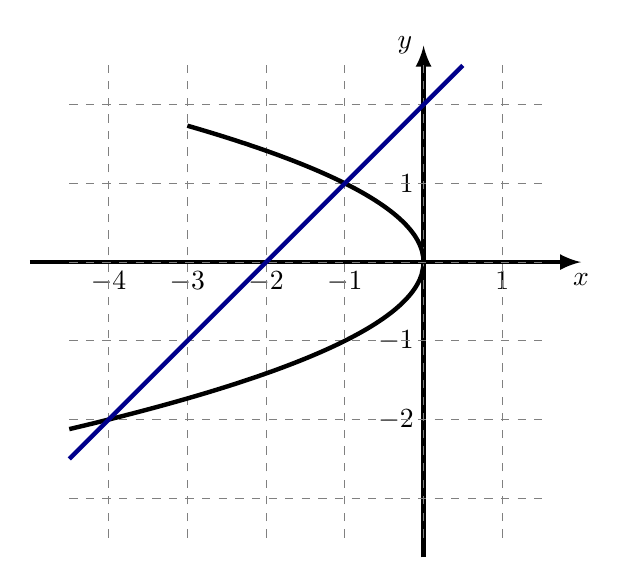
\begin{tikzpicture}[scale=1.0]
      \draw[ultra thick,->,>=latex] (-5,0)--(2,0) node[below] {$x$};
      \draw[ultra thick,->,>=latex] (0,-3.75)--(0,2.75) node[left] {$y$};
      \draw (-1,0) node[below] {$-1$};          
      \draw (-2,0) node[below] {$-2$};          
      \draw (-3,0) node[below] {$-3$};          
      \draw (-4,0) node[below] {$-4$};          
      \draw (1,0) node[below] {$1$};
      \draw (0,1) node[left] {$1$};        
      \draw (0,-1) node[left] {$-1$};
      \draw (0,-2) node[left] {$-2$};
      \draw[help lines,gray,thin,dashed] (-4.5, -3.5) grid (1.5, 2.5);
      \draw[domain=-3:0,ultra thick,samples=200] plot ({\x},{sqrt(-\x )});
      \draw[domain=-4.5:0,ultra thick,samples=200] plot ({\x},{-sqrt(-\x )});
      \draw[domain=-4.5:0.5,ultra thick,DarkBlue,samples=200] plot ({\x},{\x+2});
    \end{tikzpicture}
    \end{center}     
    The region is bounded on the \textbf{right} by $x=-y^2$, and bounded on the \textbf{left} by $x=y-2$. The region is 
    $$R = \{(x,y) \in \mathbb R^2 \, | \, -2\le y \le 1, \quad y-2 < x < -y^2\}$$
    Therefore, 
    \begin{align}
        a & = -2 \\
        b &= +1 \\
        c &= y -2 \\
        d &= -y^2 \\
        f &= 1
    \end{align}
    }
   \else

   \fi
\fi 

\ifnum \Version=7
\part The plane that passes through $P(1,3,0)$ and contains the line $x=1+t$, $y=3+3t$, $z=2+2t$ is \framebox{\strut\hspace{4cm}}. The distance between the point $P$ and the $yz$-plane is \framebox{\strut\hspace{1cm}}. 

\ifnum \Solutions=1 {\color{DarkBlue} \textit{Solutions:} There are two parts. 
\begin{itemize}
    \item The plane is parallel to direction vector of given line, $\mathbf  v = \langle 1,3,2\rangle$. Line contains $Q(1,3,2)$, so the plane is also parallel to the vector $\mathbf{PQ} = \langle 1,3,2 \rangle - \langle 1,3,0 \rangle = \langle 0,0,2 \rangle$. It would also be ok to use any scalar multiple of this. A normal to the plane is $$\mathbf n = \mathbf  v \times \mathbf {PQ} = \begin{vmatrix} i & j & k \\ 1&3&2 \\ 0&0&2\end{vmatrix} = \langle 6,-2,0\rangle = 6\mathbf i-2\mathbf j$$ So using point $P(1,3,0)$ and $\mathbf n$, the plane has equation \begin{align}
    6(x-1)+(-2)(y-3) + (0)(z-0) = 0 
\end{align}which could be simplified to other forms, such as $$3x-y=0$$ But it isn't necessary to simplify the equation. 
\item The distance between $P$ and the $yz$-plane is the $x-$coordinate, $1$.
\end{itemize}


}
\else
  
\fi
\fi


\ifnum \Version=8
    \part The average value of $f(x,y) = 12xy-16y^2$ over the region in the first quadrant bounded by $x=2$, $y=4$, and $y=4-2x$ is $\displaystyle  \int_a^b \int_c^d g(x,y) \, dx \, dy$,  where $a=\framebox{\strut\hspace{1cm}}$, $b=\framebox{\strut\hspace{1cm}}$, $c=\framebox{\strut\hspace{2cm}}$, $d=\framebox{\strut\hspace{2cm}}$, and $g(x,y) = \framebox{\strut\hspace{2cm}}$.

    \ifnum \Solutions=1 
    {\color{DarkBlue} 
    The average value of a function $f(x,y)$ over a region $R$ is given by 
    \begin{align}
        \text{Average value of }f\text{ over region }R &= \frac{1}{\text{area of region }R}\iint_R f \, dA \\&= \iint_R \frac{f(x,y)}{\text{area of region }R} \, dA
    \end{align}
    Therefore to obtain $g(x,y)$ we can calculate
    \begin{align}
        g(x,y) = \frac{f(x,y)}{\text{area of region }R}
    \end{align}
    So we need the area of the region. It can help to sketch the region, as shown in the diagram below. 
       \begin{center}     
        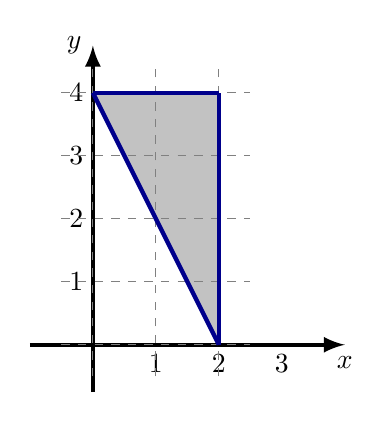
\begin{tikzpicture}[scale=0.8]
        \draw[fill=gray!80!black, opacity=0.4] (2,0) -- (2,4) -- (0,4);        
        \draw[ultra thick,->,>=latex] (-1,0)--(4,0) node[below] {$x$};
        \draw[ultra thick,->,>=latex] (0,-0.75)--(0,4.75) node[left] {$y$};
        \draw (1,0) node[below] {$1$};          
        \draw (2,0) node[below] {$2$};          
        \draw (3,0) node[below] {$3$};          
        \draw (0,1) node[left] {$1$};        
        \draw (0,2) node[left] {$2$};
        \draw (0,3) node[left] {$3$};
        \draw (0,4) node[left] {$4$};
        \draw[help lines,gray,thin,dashed] (-0.5, -0.5) grid (2.5, 4.5);
        \draw[domain=0:2,ultra thick,DarkBlue,samples=200] plot ({\x},{4-2*\x });
        \draw[domain=0:2,ultra thick,DarkBlue,samples=200] plot ({\x},{4 });
        \draw[ultra thick,-,DarkBlue,>=latex] (2,0)--(2,4);
    \end{tikzpicture}
    \end{center}     
    The region is bounded on the \textbf{right} by $y=4-2x$, or $x=2-y/2$. The region is also bounded on the \textbf{left} by $x=0$. The region is 
    $$R = \{(x,y) \in \mathbb R^2 \, | \, 0\le y \le 4, \ 0 < x < 2-y/2\}$$
    The area of the region is half the area of the rectangle whose length is 2 and height is 4. 
    $$\text{area of triangular region} = \frac12 ( 2 \cdot 4) = 4$$    
    Therefore, 
    \begin{align}
        a & = 0 \\
        b &= 4 \\
        c &= 2-y/2 \\
        d &= 2 \\
        g &= \frac{12xy-16y^2}{4} = 3xy - 4y^2
    \end{align}
    }
   \else

   \fi
\fi 



\ifnum \Version=9
\part Consider the initial value problem (IVP): $  \mathbf r ' = 4t\mathbf i + 4e^{2t}\mathbf j$, $\mathbf r(0) = 3\mathbf i + 7\mathbf j$. The solution to the IVP is $\mathbf r = \langle f(t), g(t) \rangle$, where $f(t) = \framebox{\strut\hspace{2cm}}$, $g(t) = \framebox{\strut\hspace{2cm}}$.

\ifnum \Solutions=1 {\color{DarkBlue}  \textit{Solutions:} 

\begin{align}
    f(t) &= \int 4 t \, dt = 2 t^2 +c_1 \\
    g(t) &= \int 4e^{2t} \, dt = 2e^{2t} +c_2 
\end{align}
Then using $\mathbf r(0)$, we find :
\begin{align}
    f(0) &= 3 = 0 +c_1 \\
    g(0) &= 7  = 2e^{0} +c_2 
\end{align}
So $c_1= 3$, $c_2 = 5$. So
\begin{align}
    f(t) &= 2t^2 + 3 \\
    g(t) &= 2e^{2t} + 5
\end{align}
} 
\else
  
\fi        
\fi



% 15.2
% TRIANGULAR REGION, TWO INTEGRALS TO ONE
\ifnum \Version=10
    \part $\displaystyle \int_{-2}^{2} \int_{-x}^{2} f(x,y) d y \, d x + \int_{2}^{6} \int_{x-4}^{1} f(x,y) d y \, d x = \int_{a}^{b} \int_{c}^{d} f(x,y) \, d x\,  d y$, where 
    $a=\framebox{\strut\hspace{2cm}}$, $b=\framebox{\strut\hspace{2cm}}$, $c=\framebox{\strut\hspace{2cm}}$, and $d=\framebox{\strut\hspace{2cm}}$.    

    \ifnum \Solutions=1 
    {\color{DarkBlue}
    We are given two regions: 
    \begin{align}
        R_1: &\ -2 \le x \le 2, \quad -x \le y \le 2 \\
        R_2: &\ 2 \le x \le 6, \quad x-4 \le y \le 2
    \end{align}
    The region is also
    \begin{align}
            -y \le x \le y+4, \quad -2 \le y \le 2
    \end{align}
    Thus
    \begin{align}
        V = \int_{-2}^2\int_{-y}^{y+4} f(x,y) \, dx\, dy
    \end{align}
    So,
    \begin{align}
        a=-2, \quad b = 2, \quad c=-y, \quad d = y+4
    \end{align}
    }
   \else

   \fi
\fi 







\ifnum \Version=11
    \part The position of a moving object is given by the curve $\mathbf r(t) = \langle 2+3t,4,2t^2\rangle$ for $t\in \mathbb R$. The speed of the object at $t=1$ is $\framebox{\strut\hspace{2cm}}$. A unit vector that gives the direction of motion at time $t=1$ is $\mathbf T = \langle f(t), g(t), h(t)\rangle$, where $f = \framebox{\strut\hspace{1.75cm}}$, $g = \framebox{\strut\hspace{1.75cm}}$, $h= \framebox{\strut\hspace{1.75cm}}$. 
    
    \ifnum \Solutions=1 {\color{DarkBlue} \textit{Solutions:} 
    The speed is the magnitude of the velocity. 
    \begin{align}
        \mathbf r'(t) = \mathbf v &= \langle 3,0,4t \rangle \\
        | \mathbf r'(t) | &= \sqrt{3^2+4^2t^2} \\
        | \mathbf r'(1) | &= \sqrt{25} = 5
    \end{align}
    We do not need to express the answer using any units. The unit tangent vector $\mathbf T$ gives the direction of motion at any time $t$. 
    \begin{align}
        \mathbf T 
        &= \frac{\mathbf r'(t)}{| \mathbf r'(t) |} 
        = \left\langle 
        \frac{3}{\sqrt{3+16t^2\, }},
        0,
        \frac{4t}{\sqrt{3+16t^2\,}}
        \right\rangle
    \end{align}
    Therefore,
    \begin{align}
        f(1) &= \frac{3}{5}, \quad 
        g(1) = 0, \quad 
        h(1) = \frac{4}{5} 
    \end{align}
    } 
    \else
      
    \fi        
\fi





% 15.1 EASY INTEGRATION
\ifnum \Version=12
    \part The volume of the region bounded above by $z = 2 + 3x^2 +6y^2$ and below by the rectangular region in the $xy$-plane $0\le x \le 2$, $0\le y \le 1$ is $ \int_0^{a}\int_{0}^{b} f(x,y) \, dy \, dx$ where $a=\framebox{\strut\hspace{1.5cm}}$, $b=\framebox{\strut\hspace{1.5cm}}$, $f(x,y) = \framebox{\strut\hspace{2cm}}$, and the volume of the region is $\framebox{\strut\hspace{1.5cm}}$. 
    \ifnum \Solutions=1 
    {\color{DarkBlue}
    \begin{align}
        \int_0^2\int_0^1 2 + 3x^2 +6y^2 \ dy \, dx 
        &= \int_0^2 \left. (2y +3x^2y + 2y^3 )\right|_0^1 \, dx \\ 
        &= \int_0^2  (4 + 3x^2 ) \, dx \\ 
        &= \left. (4x + x^3 )\right|_0^2 \\
        &= 16
    \end{align}
    Thus
    \begin{align}
        a &= 2 \\
        b &= 1 \\
        f &= 2 + 3x^2 +6y^2 \\ 
        \text{volume} &= 16
    \end{align}    
    }
   \else
   \fi
\fi 





\ifnum \Version=13

\part The unit tangent vector for a curve $\mathbf r(t)$ is $\mathbf T(t) = \langle 0, \cos t, \sin t \rangle$. The unit normal vector is $\mathbf  N = \langle f(t), g(t), g(t) \rangle$, where $f(t) = \framebox{\strut\hspace{2cm}}$, $g(t) = \framebox{\strut\hspace{2cm}}$, $h(t) =\framebox{\strut\hspace{2cm}}$. 

\ifnum \Solutions=1 {\color{DarkBlue} \textit{Answer:} \textit{Solutions:} The normal vector is

\begin{align}
    \mathbf N &= \frac{d\mathbf T/dt}{|d\mathbf T/dt|} 
\end{align}
And
\begin{align}
    \mathbf T'(t) &= \langle 0,-\sin t, \cos t \rangle \\
    |\mathbf T'(t) | &= \sqrt{ 0 +(-\sin t)^2 + (\cos t)^2} =1\\
    \mathbf N &= \frac{d\mathbf T/dt}{|d\mathbf T/dt|} = \langle 0, - \sin(t),  \cos(t) \rangle
\end{align}
} 
\else
\fi        
\fi



% 15.6
% BASED ON  THOMAS, 15.6 #3
% GOOD PROBLEM FOR #4, EASY
\ifnum \Version=14
    \part A thin plate of density $\delta(x,y)=2$ is bounded by $y=x-1$ and $y=5-x^2$. The plate has mass $M$, and the $y-$coordinate of the center of mass is $\bar y = M_x/M$, where $M_x = \int_a^b \int_c^d f(x,y) \, dy \, dx$,  and $b=\framebox{\strut\hspace{1.0cm}}$, $c=\framebox{\strut\hspace{2cm}}$, $d=\framebox{\strut\hspace{2cm}}$, and $f(x,y) = \framebox{\strut\hspace{2cm}}$. 

    \ifnum \Solutions=1
    {\color{DarkBlue}
    The region is bounded by 
    $$x-1 \le y \le 5-x^2$$
    The given curves intersect when 
    \begin{align}
        x-1 &= 5-x^2 \\
        0 &= x^2 +x -6 \\
        &= (x+3)(x-2)
    \end{align}
    Thus
    \begin{align}
        \bar y &= \frac{M_x}M = \frac1M \int_{-3}^{2}\int_{x-1}^{5-x^2} 2y \, dy \, dx
    \end{align} 
    The density of the plate is $\delta = 2$. Thus
    \begin{align}
        a &= -3 \\
        b &= 2 \\
        c&= x-1 \\
        d&= 5-x^2 \\
        f(x,y) &= \delta y = 2y
    \end{align}
    }
   \else
   \fi
    
\fi

